\section{Theory of association reactions}
\label{subsec:rate-theory}

The helium complex formation process is an association reaction treated here as an independent \qt{two-step} process. In this section, the equations for the overall effective binary association rate constant as described by \citet{gerlich_experimental_1992}, and \citet{bates_radiative_1988}  are simplified and derived as follows.

Initially as the first step, the ion and neutral come together to form an excited intermediate complex: 

% \[ \text{CD}^+ + \text{He} \xrightarrow{k_c} (\text{HeCD}^+) ^*\]
\begin{equation}
    \text{A}^+ + \text{B} \xrightarrow{k_c} (\text{AB}^+) ^*
\end{equation}
where $k_c$ is a bi-molecular rate constant for complex formation. The term excited intermediate complex indicates that it is a short-lived intermediate molecular ion with total internal energy above its dissociation limit and a lifetime of $\tau_{dis}$  towards dissociation::

\begin{equation}
    (\text{AB}^+) ^* \xrightarrow{k_{dis}} \text{A}^+ + \text{B}
    \label{eqn:rate-theory:decay}
\end{equation}
where $k_{dis} = \frac{1}{\tau_{dis}}$ is a first-order rate for this back-dissociation process. Under most experimental conditions Eq. \ref{eqn:rate-theory:decay} dominates but a fraction of complexes are stabilized either via emitting a photon:

\begin{equation}
    (\text{AB}^+) ^* \xrightarrow{k_{rad}} \text{AB}^+ + hv
    \label{eqn:rate-theory:via-hv}
\end{equation}
where $k_{rad}$ is a radiative rate,

or via a stabilizing collision with a neutral reactant molecule B

\begin{equation}
    (\text{AB}^+) ^* + \text{B}\xrightarrow{k_{B}} \text{AB}^+ + \text{B}
    \label{eqn:rate-theory:via-He}
\end{equation}

where $k_{B}$ is a collisional stabilization rate constant with a neutral third body B and its rate is given by $\frac{1}{\tau_B} = k_{B}$ [B] .

The overall association reaction can be summarised as:

\[ \text{A}^+ + \text{B} \xrightarrow{k_{e}} \text{AB}^+ \]
where $k_{e}$ is an overall second-order effective rate constant for the formation of the AB$^+$ stable complex which can be described as follows (while substituting B = He, i.e., helium, which is the neutral reaction partner used in this study)

\begin{equation}
    k_{e} = k_c \cdot \frac{k_{He}[He] + k_{rad}}{k_{dis} + k_{He}[He] + k_{rad}} 
    \label{eqn:rate-theory:k*}
\end{equation}

where $[He]$ indicates helium number density [in \percc].\\

Since as discussed in eq. \ref{eqn:rate-theory:decay}, $k_{dis}$ dominates over radiative and collisional stabilisation rates i.e., $k_{dis} >> k_{He}[He] + k_{rad}$, Eq. \ref{eqn:rate-theory:k*} can be simplified into the form of:
\[ k_{e} = k_c \cdot \frac{k_{He}[He] + k_{rad}}{k_{dis}} \]

which can be expressed in terms of ternary association ($k_3$) and bi-molecular radiative ($k_r$) rate constants
as shown below:

\begin{equation}
    k_3 = k_c \cdot \frac{k_{He}}{k_{dis}}
    \label{eqn:rate-theory:k3}
\end{equation}

\begin{equation}
    k_r = k_c \cdot \frac{k_{rad}}{k_{dis}}
    \label{eqn:rate-theory:kr}
\end{equation}

The final simplified overall effective binary rate constant ($k_{e}$) and rate ($R_{e}$) is expressed as:
\begin{equation}
    k_{e} = k_3[He] + k_r
    \label{eqn:rate-theory:k*-simplified}
\end{equation}

\begin{equation}
    R_{e} = k_{e}[He]
    \label{eqn:rate-theory:R*-simplified}
\end{equation}
\\\\
\textbf{Langevin rate coefficient:}\\
For ion-neutral reactions, the Langevin rate coefficient, $k_L$, is a classical theoretical reaction rate coefficient given by \citet{langevin_notitle_1905}.  The final equation for $k_L$, with an ion of charge $q$ [in $C$], ion-neutral reduced mass $\mu$ [in amu] and polarizability of the neutral $\alpha$ [in $\mathring{\text{A}}^3$], summarised by \citet{asvany_numerical_2009}, is given as:
\label{discussions:Langevin}

\begin{equation}
    \begin{split}
        k_L [\text{cm}^3 / \text{s}] & = q \sqrt{\frac{\pi \alpha}{\epsilon _0 \mu}} \\
        &= 2.342 \cdot \sqrt{ \frac{\alpha}{\mu}} \cdot 10^{-9} 
   \end{split}
   \label{eqn:Langevin}
\end{equation}


The Langevin rate coefficient, $k_L$, for the \CD + He reaction can be calculated from Eq. \ref{eqn:Langevin} by substituting helium polarizability, $\alpha=0.208\  \mathring{\text{A}}^3$ \cite{olney_absolute_1997} and He\CD pair reduced mass $\mu=3.11$ amu:

\begin{equation}
        k_L = 6.06 \cdot 10^{-10} \text{ cm}^3 / \text{s}.
   \label{eqn:Langevin-CD+}
\end{equation}
\\
\textbf{He\CD binding energy:}\label{discussions:binding-energy:CD+}\\

\begin{figure}[!htb]
    \centering
    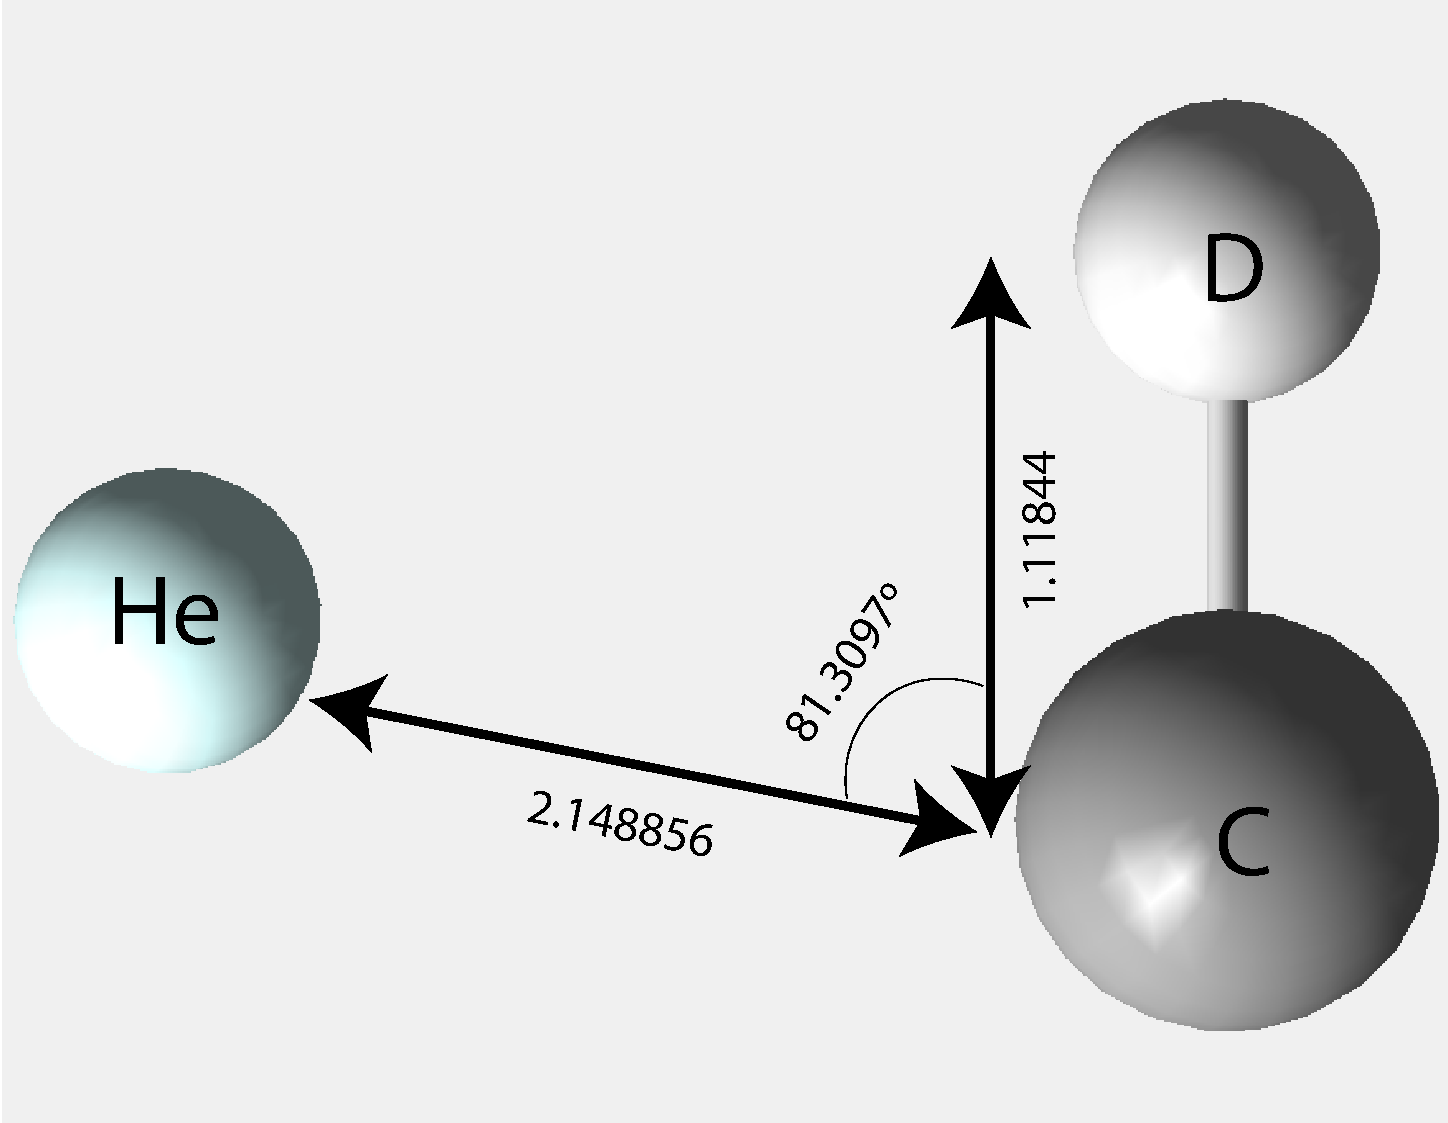
\includegraphics[width=0.5\textwidth]{figures/measurements/kinetics/HeCD+_geometry.pdf}
    \caption{He\CD optimized geometry computed at the CCSD(T)/aug-cc-pVTZ level of theory.}
    \label{fig:HeCD_geometry}
\end{figure}

The He\CD geometry was optmised at the CCSD(T)/aug-cc-pVTZ level of theory. The computed geometry is shown in Figure \ref{fig:HeCD_geometry}.
The computed binding energy of He\CD is $D_e=491$ \wnn at this level of theory. The binding energy is counterpoise corrected for the basis set superposition error (BSSE) \cite{boys_calculation_1970}.
\citet{stoecklin_vibrational_2008} computed BSSE corrected $D_e=513.573$ \wnn for HeCH$^+$ complex using BCCSD(T) /aug-cc-PVQZ method.
The binding energy is not zero-point energy corrected.

% The relationship between the dissociation rate ($k_{CID}$), Langevin rate ($k_L$) and binding energy ($D_0$) is given by \cite{SGA2015}:

% \begin{equation}
%     k_{CID} = k_L \cdot \text{exp} \left( \frac{-D_0}{k_B \cdot T_{coll}} \right)
%     \label{eqn:relation:kCID-kL} 
% \end{equation}

% By substiting the expression for $k_L=6 \cdot 10^{-10}$ \pers\ (see Section \ref{discussions:Langevin}), 
% $k_{CID}=5.3 \cdot 10^{-16}$ \pers\ (see Table \ref{tab:kCID:rate-constants}), $k_B=0.6950$ \wnn 
% and T$_{coll}=7.1$ K in Eq. \ref{eqn:relation:kCID-kL}, we get:

% \begin{equation}
%     D_0 = 69 \text{ cm}^{-1}
% \end{equation}